\documentclass[14pt]{article}

\usepackage[utf8x]{inputenc}
\usepackage[russian]{babel}
\usepackage{graphicx}
\graphicspath{{images/}}
\DeclareGraphicsExtensions{.pdf,.png,.jpg}

\usepackage{amsmath}
\usepackage{pgfplots}

\usepackage{geometry} % Меняем поля страницы
\geometry{left=2cm}% левое поле
\geometry{right=1.5cm}% правое поле
\geometry{top=2cm}% верхнее поле
\geometry{bottom=2cm}% нижнее поле

\renewcommand{\theenumi}{\arabic{enumi}}
\renewcommand{\labelenumi}{\arabic{enumi}}
\renewcommand{\theenumii}{.\arabic{enumii}}
\renewcommand{\labelenumii}{\arabic{enumi}.\arabic{enumii}.}
\renewcommand{\theenumiii}{.\arabic{enumiii}}
\renewcommand{\labelenumiii}{\arabic{enumi}.\arabic{enumii}.\arabic{enumiii}.}

\begin{document}
\begin{titlepage}
	\begin{center}
		\fontsize{18pt}{20pt}\selectfont
		\textbf{Работа 3.3.5.}	
	
		\vspace{5cm}
		\fontsize{24pt}{25pt}\selectfont
		Эффект Холла в металлах
	\end{center}
	\begin{flushright}
		\fontsize{18pt}{20pt}\selectfont
		\vspace{14cm}
		\hspace{-3cm}
		\textit{Корнеев Е.С.}
	\end{flushright}		
\end{titlepage}

\begin{center}
	\fontsize{16pt}{18pt}\selectfont	
	Эффект Холла в металлах
\end{center}


\fontsize{14pt}{16pt}\selectfont
\vspace{1cm}
\textbf{Цель работы:} измерение подвижности и концентрации носителей заряда в металлах.

\vspace{0.5cm}
\textbf{Оборудование:} электромагнит с источником питания, источник постоянного тока, микровольтметр, амперметры, измеритель магнитной индукции, образцы из серебра и цинка. 

\vspace{1cm}
Суть эффекта Холла заключается в следующем: пусть через однородную пластину металла вдоль оси $x$ течет ток $I$. Если поместить пластину в однородное магнитное поле $B$, направленное по $y$, то между гранями $A$ и $\text{Б}$ появится разность потенциалов. Действительно, на движущийся с 
$\langle\vec{v}\rangle$ заряд будет действовать сила Лоренца
$$
	\vec{F_{\text{Л}}} = -e\vec{E} - e\langle\vec{v}\rangle \times \vec{B}
$$
\noindent где $e$ - абсолютная величина заряда, $\vec{E}$ - напряженность электрического поля, $\vec{B}$ - индукция магнитного поля. 

\begin{figure}[h!]
	\center{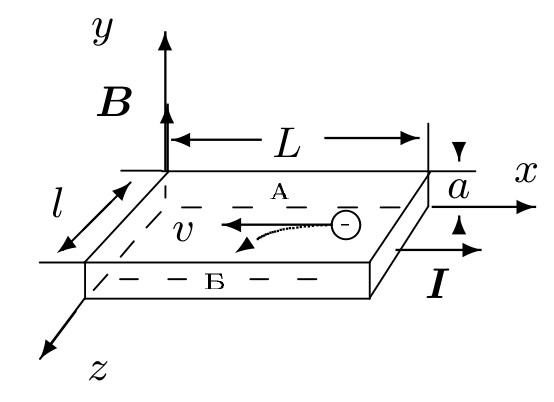
\includegraphics[width = 10cm]{Hall}}
	\caption{Эффект Холла}
	\label{fig:image}
\end{figure}

В нашем случае сила, обусловленная вторым слагаемым, направлена вдоль $z$ и равна 
$$
	F_B = e|\langle v_x\rangle|B
$$
\noindent где $|\langle v_x\rangle|$ - дрейфовая скорость заряда вдоль оси $x$. Под действием силы $F_B$ электроны отклоняются к грани 
$\text{Б}$, заряжая ее отрицательно, а на грани А накапливаются нескомпенсированные положительные заряды, из-за чего возникает электрическое поле $E_z$, направленное вдоль оси $z$. Его действие на заряды можно описать уравнением $F_{E_z} = eE_z$, причем сила $F_{E_z}$ дейстует против силы $F_B$. Через некоторое время наступает установившийся режим, когда накопление зарядов прекращается и $F_{E_z} = F_B$. Отсюда нетрудно получить
$$
	E_z = |\langle v_x\rangle|B
$$

С полем $E_z$ связана разность потенциалов $U_{\text{АБ}}$:
$$
	U_{\text{АБ}} = -E_zl = -|\langle v_x\rangle|Bl
$$

В этом и состоит эффект Холла. Замечая, что $I = ne|\langle v_x\rangle|la$, получим
$$
	\varepsilon_{\text{АБ}} = U_{\text{АБ}} = -\frac{IB}{nea} = -R_x\cdot\frac{IB}{a}
$$

Константа $R_x$ называется \textsl{постоянной Холла}:
$$
	R_x = \frac{1}{ne}
$$

\vspace{1cm}
\textbf{Экспериментальная установка} 

\begin{figure}[h!]
	\center{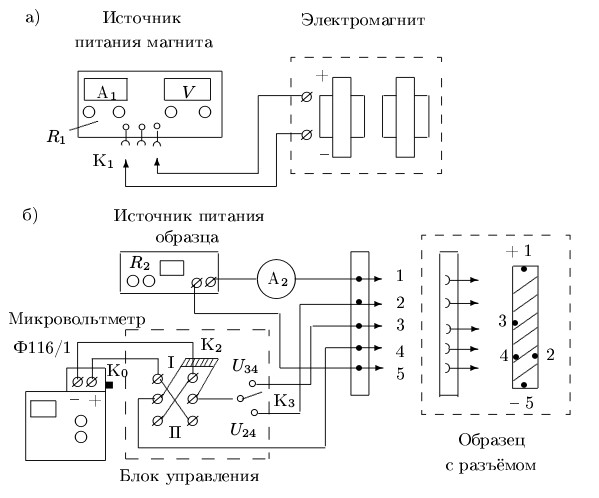
\includegraphics[width = 13cm]{facility}}
	\caption{Экспериментальная установка}
	\label{fig:image}
\end{figure}

В зазоре электромагнита создается постоянное магнитное поле, величину которого можно менять с помощью источника питания. Направление тока можно менять, переключая ключ $K_1$, ток через электромагнит измеряется амперметром $A_1$. Перед использование электромагнита проградуируем его при помощи милливеберметра. Ток через металлические образцы в форме пластинок регулируется реостатом $R_2$ и измеряется амперметром $A_2$. ЭДС Холла измеряется микровольтметром.

Вследствие неточности подпайки контактов к образцу не лежат на одной эквипотенциали, вследствие чего напряжение между ними связано не только с эффектом Холла, но и с омическим падением напряжения. Чтобы исключить это сопротивление, будем измерять напряжение $U_0$ между контактами образца в отсутствие магнитного поля, и затем вычетать это значение из снимаемого напряжения. 

\vspace{1cm}
\textbf{Ход работы.}

0. Определим геометрические размеры образцов:

\begin{center}
\begin{tabular}{|c|c|c|c|c|c|c|}
\hline
			&	$L$, мм		&	$a$, мм		&	$l$, мм		\\
\hline
серебро		&	15.0		&	0.09		&	11.0		\\
\hline
цинк		&	3.5			&	0.12		&	10.5		\\
\hline
\end{tabular}
\end{center}

1. Проградуируем электромагнит, сняв зависимость $B(I)$:

\begin{center}
\begin{tabular}{|c|c|c|c|c|}
\hline
$I$, А		&		$B$, мТл	\\
\hline
0.1			&		111			\\
\hline
0.2			&		211			\\
\hline
0.4			&		424			\\
\hline
0.6			&		618			\\
\hline
0.8			&		799			\\
\hline
1.0			&		937			\\
\hline
1.1			&		1006		\\
\hline
1.2			&		1038		\\
\hline
1.3			&		1080		\\
\hline
1.4			&		1113		\\
\hline
1.5			&		1129		\\
\hline
\end{tabular}
\end{center}

\begin{flushleft}
\begin{tikzpicture}
\begin{axis}[
	height = 9cm,
	width  = 14cm,
	every axis y label/.style={at = {(ticklabel cs: 0.5)}, rotate = 90, anchor = near ticklabel},
	xlabel = {$I$, А},
	ylabel = {$B$, мТл}
]
\addplot+[%error bars/.cd, 
	%y dir = both, y explicit,
	%x dir = both, x explicit,
	only marks
	]
coordinates{
	%(0,0)
	(0.1 , 111 )
	(0.2 , 211 )
	(0.4 , 424 )
	(0.6 , 618 )
	(0.8 , 799 )
	(1.0 , 937 )
	(1.1 , 1006)
	(1.2 , 1038)
	(1.3 , 1080)
	(1.4 , 1113)
	(1.5 , 1129)
};

\addplot+[
	blue,
	smooth,
	mark = none
	]
coordinates{
	%(0,0)
	(0.1 , 111 )
	(0.2 , 211 )
	(0.4 , 424 )
	(0.6 , 618 )
	(0.8 , 799 )
	(1.0 , 940 )
	(1.1 , 1000)
	(1.2 , 1050)
	(1.3 , 1085)
	(1.4 , 1113)
	(1.5 , 1129)
};

\end{axis}
\end{tikzpicture}
\end{flushleft}


2. Теперь снимем зависимости $U(I_M)$ для разных значениях тока $I$ через серебряный образец:

\vspace{1cm}
\begin{tabular}{|c|c|c|c|c|c|c|c|c|c|c|c|c|c|c|c|}
\hline
\multicolumn{3}{|c|}{$I = 0.2$ A}			&	\multicolumn{3}{|c|}{$I = 0.4$ A}			&	\multicolumn{3}{|c|}{$I = 0.6$ A}			\\
\hline
$I_M$, А	&	$U$, дел	&	$U$, мкВ	&	$I_M$, А	&	$U$, дел	&	$U$, мкВ	&	$I_M$, А	&	$U$, дел	&	$U$, мкВ	\\
\hline
0.0			&	1			&				&	0.0			&	0			&				&	0.0			&	-1			&				\\
\hline
0.2			&	2			&	0.04		&	0.2			&	1			&	0.04		&	0.2			&	2			&	0.12		\\
\hline
0.4			&	3			&	0.08		&	0.4			&	3			&	0.12		&	0.4			&	5			&	0.24		\\
\hline
0.6			&	4			&	0.12		&	0.6			&	4			&	0.16		&	0.6			&	7			&	0.32		\\
\hline
0.8			&	5			&	0.16		&	0.8			&	6			&	0.24		&	0.8			&	10			&	0.44		\\
\hline
1.0			&	5			&	0.16		&	1.0			&	7			&	0.28		&	1.0			&	11			&	0.48		\\
\hline
1.2			&	6			&	0.20		&	1.2			&	8			&	0.32		&	1.2			&	13			&	0.56		\\
\hline
1.4			&	6			&	0.20		&	1.4			&	8			&	0.32		&	1.4			&	13			&	0.56		\\
\hline
\end{tabular}

\vspace{0.5cm}
\begin{tabular}{|c|c|c|c|c|c|c|c|c|c|c|c|c|c|c|c|}
\hline
\multicolumn{3}{|c|}{$I = 0.8$ A}			&	\multicolumn{3}{|c|}{$I = 1.0$ A}			&	\multicolumn{3}{|c|}{$I = 1.2$ A}			\\
\hline
$I_M$, А	&	$U$, дел	&	$U$, мкВ	&	$I_M$, А	&	$U$, дел	&	$U$, мкВ	&	$I_M$, А	&	$U$, дел	&	$U$, мкВ	\\
\hline
0.0			&	-1			&				&	0.0			&	-1			&				&	0.0			&	-1			&				\\
\hline
0.2			&	2			&	0.12		&	0.2			&	3			&	0.16		&	0.2			&	4			&	0.20		\\
\hline
0.4			&	6			&	0.28		&	0.4			&	8			&	0.36		&	0.4			&	10			&	0.44		\\
\hline
0.6			&	9			&	0.40		&	0.6			&	12			&	0.52		&	0.6			&	15			&	0.64		\\
\hline
0.8			&	13			&	0.56		&	0.8			&	17			&	0.72		&	0.8			&	20			&	0.84		\\
\hline
1.0			&	15			&	0.64		&	1.0			&	20			&	0.84		&	1.0			&	24			&	1.00		\\
\hline
1.2			&	16			&	0.68		&	1.2			&	22			&	0.92		&	1.2			&	26			&	1.08		\\
\hline
1.4			&	18			&	0.76		&	1.4			&	23			&	0.96		&	1.4			&	28			&	1.16		\\
\hline
\end{tabular}

\vspace{1cm}
Обратное направление вектора магнитной индукции:

\begin{center}
\begin{tabular}{|c|c|c|c|c|c|c|c|c|c|c|c|c|c|c|c|}
\hline
\multicolumn{3}{|c|}{$I = 1.2$ A}			\\
\hline
$I_M$, А	&	$U$, дел	&	$U$, мкВ	\\
\hline
0.0			&	6			&				\\
\hline
0.2			&	10			&	0.16		\\
\hline
0.4			&	17			&	0.44		\\
\hline
0.6			&	22			&	0.64		\\
\hline
0.8			&	28			&	0.88		\\
\hline
1.0			&	32			&	1.04		\\
\hline
1.2			&	35			&	1.16		\\
\hline
1.4			&	38			&	1.28		\\
\hline
\end{tabular}
\end{center}


\vspace{1cm}
Пересчет из делений в милливольты осуществлялся исходя из соотношения 1 дел = 0.04 мкВ в данном режиме. Значение $U_0$ записано в первой строке для каждой из таблиц ($I_M = 0$), пересчет из делений в мВ осуществляется уже после вычитания $U_0$ из измеряемого напряжения. Погрешность приборную $\sigma_U$ примем равной 0.02 мкВ, на ее фоне погрешностью силы тока $\sigma_I$, равно как и погрешностью $\sigma_B$, можно пренебречь. 


3. Имея зависимость $B(I_M)$, получим зависимости $\varepsilon(B)$:

\begin{center}
\begin{tabular}{|c|c|c|c|c|c|c|c|c|c|c|c|c|c|c|c|}
\hline
\multicolumn{2}{|c|}{$I = 0.2$ A}			&	\multicolumn{2}{|c|}{$I = 0.4$ A}			&	\multicolumn{2}{|c|}{$I = 0.6$ A}			\\
\hline
$U$, мкВ	&	$B$, мТл					&	$U$, мкВ	&	$B$, мТл					&	$U$, мкВ	&	$B$, мТл					\\
\hline
0.04		&	210							&	0.04		&	210							&	0.12		&	210							\\
\hline
0.08		&	420							&	0.12		&	420							&	0.24		&	420							\\
\hline
0.12		&	620							&	0.16		&	620							&	0.32		&	620							\\
\hline
0.16		&	800							&	0.24		&	800							&	0.44		&	800							\\
\hline
0.16		&	940							&	0.28		&	940							&	0.48		&	940 						\\
\hline
0.20		&	1010						&	0.32		&	1010						&	0.56		&	1010						\\
\hline
0.20		&	1040						&	0.32		&	1040						&	0.56		&	1040						\\
\hline
\end{tabular}
\end{center}

\begin{center}
\begin{tabular}{|c|c|c|c|c|c|c|c|c|c|c|c|c|c|c|c|}
\hline
\multicolumn{2}{|c|}{$I = 0.8$ A}			&	\multicolumn{2}{|c|}{$I = 1.0$ A}			&	\multicolumn{2}{|c|}{$I = 1.2$ A}			\\
\hline
$U$, мкВ	&	$B$, мТл					&	$U$, мкВ	&	$B$, мТл					&	$U$, мкВ	&	$B$, мТл					\\
\hline
0.12		&	210							&	0.16		&	210							&	0.20		&	210							\\
\hline
0.28		&	420							&	0.36		&	420							&	0.44		&	420							\\
\hline
0.40		&	620							&	0.52		&	620							&	0.64		&	620							\\
\hline
0.56		&	800							&	0.74		&	800							&	0.84		&	800							\\
\hline
0.64		&	940							&	0.84		&	940							&	1.00		&	940 						\\
\hline
0.68		&	1010						&	0.92		&	1010						&	1.08		&	1010						\\
\hline
0.76		&	1040						&	0.96		&	1040						&	1.16		&	1040						\\
\hline
\end{tabular}
\end{center}

\vspace{1cm}
Таким образом, получаем семейство графиков:

\begin{flushleft}
\begin{tikzpicture}
\begin{axis}[
	height = 10cm,
	width  = 16cm,
	every axis y label/.style={at = {(ticklabel cs: 0.5)}, rotate = 90, anchor = near ticklabel},
	xlabel = {$B$, мТл},
	ylabel = {$\varepsilon$, мкВ},
	xmin = 0,
	ymin = 0
]

%%%%%%%%%%%%%%%%%%%%%%%%%%%%%%%%%%%%%%%%

\addplot+[
	only marks,
	]
coordinates{
	(210 , 0.04)
	(420 , 0.08)	
	(620 , 0.12)	
	(800 , 0.16)	
	(940 , 0.16)	
	(1010, 0.20)	
	(1040, 0.20)	
};

\addplot [mark = none]
coordinates{
	(0, -0.00176168)
	(1040, 0.203846)
};

%%%%%%%%%%%%%%%%%%%%%%%%%%%%%%%%%%%%%%%%

\addplot+[
	only marks,
	]
coordinates{
	(210 , 0.04)
	(420 , 0.12)
	(620 , 0.16)
	(800 , 0.24)	
	(940 , 0.28)
	(1010, 0.32)
	(1040, 0.32)
};

\addplot [mark = none]
coordinates{
	(0, 0)
	(1040, 0.312034)
}; 

%%%%%%%%%%%%%%%%%%%%%%%%%%%%%%%%%%%%%%%%

\addplot+[
	only marks,
	]
coordinates{
	(210 , 0.12)
	(420 , 0.24)
	(620 , 0.32)
	(800 , 0.44)
	(940 , 0.48)
	(1010, 0.56)
	(1040, 0.56)
};

\addplot [mark = none]
coordinates{
	(0, 0.00881752)
	(1040, 0.557351)
};


%%%%%%%%%%%%%%%%%%%%%%%%%%%%%%%%%%%%%%%%

\addplot+[
	only marks,
	]
coordinates{
	(210 , 0.12)
	(420 , 0.28)
	(620 , 0.40)
	(800 , 0.56)
	(940 , 0.64)	% 68
	(1010, 0.68)	% 76
	(1040, 0.76)	% 80
};

\addplot [mark = none]
coordinates{
	(0, -0.0243989)
	(1050, 0.70)
};

%%%%%%%%%%%%%%%%%%%%%%%%%%%%%%%%%%%%%%%%

\addplot+[
	only marks,
	]
coordinates{
	(210 , 0.16)
	(420 , 0.36)
	(620 , 0.52)
	(800 , 0.74)
	(940 , 0.84)	
	(1010, 0.92)	%96	
	(1040, 0.96)	%104
};

\addplot [mark = none]
coordinates{
	(0, -0.0472127)
	(1040, 0.949555)
};

%%%%%%%%%%%%%%%%%%%%%%%%%%%%%%%%%%%%%%%%

\addplot+[
	only marks,
	]
coordinates{
	(210 , 0.20)
	(420 , 0.44)
	(620 , 0.64)
	(800 , 0.84)
	(940 , 1.00)	
	(1010, 1.08)	% 112
	(1040, 1.16)	% 124
};

\addplot [mark = none]
coordinates{
	(0, -0.040724)
	(1040, 1.12413)
};

\end{axis}
\end{tikzpicture}
\end{flushleft}


\vspace{1cm}
Определим $k = \Delta\varepsilon/\Delta B$ по МНК:

\begin{center}
\begin{tabular}{|c|c|c|c|c|c|c|c|c|c|}
\hline
$I$, А		&	$k$, В/Тл$\cdot 10^{-6}$	&	$\sigma_k$, В/Тл$\cdot 10^{-6}$	\\
\hline
0.2			&	0.20						&	0.01								\\
\hline
0.4			&	0.34						&	0.02								\\
\hline
0.6			&	0.53						&	0.03								\\
\hline
0.8			&	0.71						&	0.03								\\
\hline
1.0			&	0.96						&	0.01								\\
\hline
1.2			&	1.12						&	0.01								\\
\hline
\end{tabular}
\end{center}


\begin{flushleft}
\begin{tikzpicture}
\begin{axis}[
	height = 10cm,
	width  = 16cm,
	every axis y label/.style={at = {(ticklabel cs: 0.5)}, rotate = 90, anchor = near ticklabel},
	xlabel = {$I$, А},
	ylabel = {$k$, В/Тл$\cdot 10^{-8}$},
	xmin = 0,	
	ymin = 0
]
\addplot+[
	only marks,
	error bars/.cd, 
	y dir = both, y explicit,
	x dir = both, x explicit,
	]
coordinates{
	(0.2, 20 )	+- (0, 1)
	(0.4, 34 )	+- (0, 2)
	(0.6, 53 )	+- (0, 3)
	(0.8, 71 )	+- (0, 3)
	(1.0, 96 )	+- (0, 1)
	(1.2, 112)	+- (0, 1)
};

\addplot [mark = none]
coordinates{
	(0, -2.06667)
	(1.2, 111.762)
};

\end{axis}
\end{tikzpicture}
\end{flushleft}

Теперь определим угловой коэффициент по МНК, пользуясь формулами:
$$
	k = \frac{\langle xy\rangle - \langle x\rangle\langle y\rangle}{\langle x^2\rangle - \langle x\rangle^2},
$$
$$
	\sigma_k \approx \frac{1}{\sqrt{n}}\sqrt{\frac{\langle y^2\rangle - \langle y\rangle^2}{\langle x^2\rangle - \langle x\rangle^2} - k^2},
$$
\noindent где предполагается линейная заивисимость $y = kx + b$. Таким образом, $\Delta k/\Delta I = 95\cdot 10^{-8} \frac{\text{В}}{\text{А}\cdot\text{Тл}}$. Зная его, получаем 
$$
	R_x = -k\cdot a = -0.86 \cdot 10^{-10} \frac{\text{м}^3}{\text{Кл}}
$$
Определим по МНК случайную погрешность:
$$
	\sigma_{\text{случ}} = 0.02 \cdot 10^{-10}\frac{\text{м}^3}{\text{Кл}}
$$
Приборную оценим по формуле 
$$
	\sigma_{\text{приб}} = \sqrt{\left(\sum_{i = 0}^n \frac{\partial f}{\partial x_i}\sigma_{x_i}\right)^2},
$$
\noindent считая $R_x$ функцией от $U, I$:
$$
	\sigma_{\text{приб}} \approx 0.04 \cdot 10^{-10}\frac{\text{м}^3}{\text{Кл}}
$$
\noindent тогда 
$$
	\sigma_{R_x} = \sqrt{\sigma_{\text{приб}}^2 + \sigma_{\text{случ}}^2} = 0.04 \cdot 10^{-10} \frac{\text{м}^3}{\text{Кл}}
$$
\noindent или
$$
	\boxed{R_x^{\text{серебро}} = (-0.84 \pm 0.04) \cdot 10^{-10} \frac{\text{м}^3}{\text{Кл}}}
$$

\vspace{1cm}
4. Построим аналогичные зависимости для цинкового образца.

Соответствующая зависимость для образца из цинка:

\begin{center}
\begin{tabular}{|c|c|c|c|c|c|c|c|c|c|c|c|c|c|c|c|}
\hline
\multicolumn{4}{|c|}{$I = 1.0$ A}							\\
\hline
$I_M$, А	&	$U$, дел	&	$U$, мкВ	&	$B$, мТл	\\
\hline
0.0			&	13			&				&				\\
\hline
0.2			&	19			&	0.24		&	210			\\
\hline
0.4			&	24			&	0.44		&	420			\\
\hline
0.6			&	29			&	0.64		&	620			\\
\hline
0.8			&	34			&	0.84		&	800 		\\
\hline
1.0			&	38			&	1.00		&	940 		\\
\hline
1.2			&	40			&	1.08		&	1010		\\
\hline
1.4			&	42			&	1.16		&	1040		\\
\hline
\end{tabular}
\end{center}

\vspace{1cm}
\begin{flushleft}
\begin{tikzpicture}
\begin{axis}[
	height = 10cm,
	width  = 16cm,
	every axis y label/.style={at = {(ticklabel cs: 0.5)}, rotate = 90, anchor = near ticklabel},
	xlabel = {$B$, мТл},
	ylabel = {$\varepsilon$, мкВ},
	xmin = 0,
	ymin = 0
]

\addplot+[
	only marks,
	]
coordinates{
	(210 , 0.24)
	(420 , 0.44)
	(620 , 0.64)
	(800 , 0.84)
	(940 , 1.00)	
	(1010, 1.08)
	(1040, 1.16)
};

\addplot [mark = none]
coordinates{
	(0, -0.0105867)
	(1040, 1.11899)
};

\end{axis}
\end{tikzpicture}
\end{flushleft}


Аналогично найдем угловой коэффициент и определим его погрешность, используя МНК:
$$
	k = \frac{\Delta\varepsilon}{\Delta B} = 108 \cdot 10^{-8} \frac{\text{В}}{\text{Тл}}
$$
$$
	\sigma_{\text{случ}} = 3 \cdot 10^{-8} \frac{\text{В}}{\text{Тл}}
$$
\noindent Считая $k = f(U, I)$:
$$
	\sigma_{\text{приб}} \approx 5 \cdot 10^{-8} \frac{\text{В}}{\text{Тл}}
$$
\noindent Отсюда получаем:
$$
	\sigma_{k} = \sqrt{\sigma_{\text{приб}}^2 + \sigma_{\text{случ}}^2} = 6 \cdot 10^{-8} \frac{\text{В}}{\text{Тл}}
$$

Таким образом:
$$
	k = (108 \pm 6)\cdot 10^{-8} \frac{\text{В}}{\text{Тл}}
$$
	
Отсюда несложно получить:
$$
	\boxed{R_x^{\text{цинк}} = - k\cdot\frac{a}{I} = (-1.30 \pm 0.07) \cdot 10^{-10} \frac{\text{В}}{\text{Тл}}}
$$

\vspace{1cm}
5. Определим напряжения $U_{34}$ для серебра и цинка в отсутствие магнитного поля:

\begin{center}
\begin{tabular}{|c|c|c|c|c|c|c|c|c|c|c|}
\hline
			&	$U_{34}$, дел	&	$U_{34}$, мкВ	\\
\hline
серебро		&	27				&	270				\\
\hline
цинк		&	24				&	240 			\\
\hline
\end{tabular}
\end{center}

В данном режиме измерений 75 делениям соответствовало 750 мкВ, откуда 1 дел = 10 мкВ. Отсюда погрешность $\sigma_{U_{34}}$ примем равной 5мкВ. Тогда можем найти удельные проводимости по формуле
$$
	\sigma = \frac{IL_{34}}{U_{34}al}:
$$
$$
	\sigma^\text{серебро} = (56.1 \pm 1.0)\cdot 10^{6} \frac{\text{Ом}}{\text{м}}
$$
$$
	\sigma^\text{цинк} = (11.5 \pm 0.2)\cdot 10^{6} \frac{\text{Ом}}{\text{м}}
$$

Определим $n$, зная значение постоянной Холла:
$$	
	n = -\frac{1}{R_xq} = -\frac{1}{R_xe}
$$
\noindent При этом погрешность можно определить, считая $n = f(R)$:
$$
	n^{\text{серебро}} = (0.74 \pm 0.04) \cdot 10^{29} \text{м}^{-3}
$$
$$
	n^{\text{цинк   }} = (0.48 \pm 0.03) \cdot 10^{29} \text{м}^{-3}
$$

\vspace{1cm}
6. Теперь, зная основной тип носителей заряда и их концентрацию, можем найти подвижность:
$$
	\sigma = enb ~~\Rightarrow ~~b = \frac{\sigma}{en},
$$
$$
	\Delta b = \sqrt{\left(\frac{\partial f}{\partial n}\sigma_n\right)^2 + \left(\frac{\partial f}{\partial\sigma}\Delta\sigma\right)^2}
$$

$$
	b^{\text{серебро}} = (47 \pm 3) \frac{\text{см}^2}{\text{В}\cdot\text{с}}
$$
$$
	b^{\text{цинк   }} = (15 \pm 3) \frac{\text{см}^2}{\text{В}\cdot\text{с}}
$$

\vspace{1cm}
Таким образом, в данной лабораторной работе мы определили концентрацию носителей зарядов в металлах, таких как серебро и цинк, а также исследовали проявления эффекта Холла в этих металлах. 


\end{document}